\documentclass{manual}
\usepackage{epsfig}
% \usepackage{pdfsync}
\usepackage{amsfonts}
\release{0.0}



\begin{document}

\title{The GaussianProcess package}
\author{Anand Patil}
\maketitle
\tableofcontents

\chapter{Introduction}\label{cha:introduction} % (fold)

Gaussian processes (GPs) are probability distributions for functions. They're useful if a functional form is unknown a priori.

GPs are not hard to understand at a conceptual level, but implementing them on a computer can require fairly involved linear algebra. This makes it hard for beginners to get started, and even when you have experience it's annoying.

This package provides Python classes that represent the components of the Gaussian process. They are meant to support many types of Gaussian process usage, from intuitive exploration to high-performance deployment in MCMC, with smooth transitions between.

The package also provides a class which produces Gaussian process-valued PyMC parameters and a PyMC sampling method to handle it. That means the Gaussian process-related objects can be directly incorporated into larger probability models.

You'll need to understand Python, numpy and a little bit of Bayesian statistics. Refs.

% chapter introduction (end)



\chapter{Installation}\label{cha:installation} % (fold)

\section{Dependencies}
\begin{itemize}
	\item \citetitle[www.python.org]{Python version 2.4} or later.
	\item \citetitle[www.scipy.org]{numpy}, Numerical Python. The core package for numerical work in Python.
	\item Optional: \citetitle[www.matplotlib.org]{matplotlib/ pylab}, Matlab-like scientific plotting utilities for Python. Install this if you want to use any of the graphical functionality described in this manual.
	\item Optional: \citetitle[www.trichech.us]{PyMC}, Bayesian statistics and MCMC support for Python. Install this if you want to embed Gaussian processes in larger probability models.
\end{itemize} 

\section{How to install}\label{sec:installing}

Type this into a shell:
\begin{verbatim}
	python setup.py install
\end{verbatim}

% chapter installation (end)



\chapter{Tutorial I: The basics}\label{cha:basics} % (fold)

% chapter basics (end)

To understand GPs, you need to play around with them. You can be as good at math as you want, but to really know what they're like you have to build experience. For that reason, after a brief overview of what GP's can be good for, this tutorial will immediately show you how to actually instantiate a GP. That way you have one to play around with throughout the rest of the tutorial. All the code in the tutorial is in the folder \file{examples}, which is distributed with this package.

Sections \ref{sec:firstlook} through \ref{sec:observing} will give you the bare minimum you need to know to get started; section \ref{sec:array} is highly recommended. Section \ref{sec:PyMC} will tell you how to incorporate your GPs into larger probability models using PyMC. The remaining sections cover more advanced topics, and are referenced at appropriate points from the introductory sections.

\section{Prerequisites}\label{sec:prerequisites}
You need to know a bit about Python and numpy. Also a bit about Bayesian statistics and the normal distribution. Refs. 

\section{A first look at Gaussian processes}\label{sec:firstlook} % (fold)

Gaussian processes are probability distributions for functions. The statement `$f$ has a Gaussian process distribution with mean $M$ and covariance $C$' is usually written as follows:
\begin{equation}
    f\sim\textup{GP}(M,C).
\end{equation}
Gaussian processes have two parameters, which are analogous to the parameters of the normal distribution:
\begin{itemize}
    \item $M$ is the mean function. Like the mean parameter of the normal distribution, $M$ gives the central tendency for $f$. In Bayesian statistics, $M$ is usually considered a prior guess for $f$. $M(x)$ gives the expectation of $f(x)$.
    \item $C$  is the covariance function. Its role is harder to understand than that of the mean function, but among other things it regulates:
    \begin{itemize}
        \item the amount by which $f$ may deviate from $M$
        \item the smoothness of $f$
        \item the wiggliness of $f$.
    \end{itemize}
    $C(x,y)$ gives the covariance of $f(x)$ and $f(y)$; $C(x,x)$ gives the variance of $f(x)$.
\end{itemize}
An intuitive understanding of covariance functions is essential for appropriate application of Gaussian processes, but for the time being don't worry about them too much. Section \ref{sec:cov} is all about covariance functions.


\subsection{What are Gaussian processes good for?}\label{sub:applications}
\textbf{Need to collect some applications. I was thinking Steve and Thanasis' Bayesian nonparametric stock recruitment paper, and possibly an actual spatial statistical application.}

\subsection{Instantiating a Gaussian process}\label{sub:inst}

The rest of this tutorial will be much easier to understand with an actual Gaussian process in hand to experiment with. The \module{GaussianProcess} module supports multivariate as well as univariate GP's; the variables $x$ and $y$ in section \ref{sec:firstlook} can be vectors just as well as scalars. For the time being, however, let's concentrate on univariate GP's, as they're easier to visualize.

\subsubsection{Instantiating a covariance function}\label{subsub:cov}
\begin{figure}
	\centering
		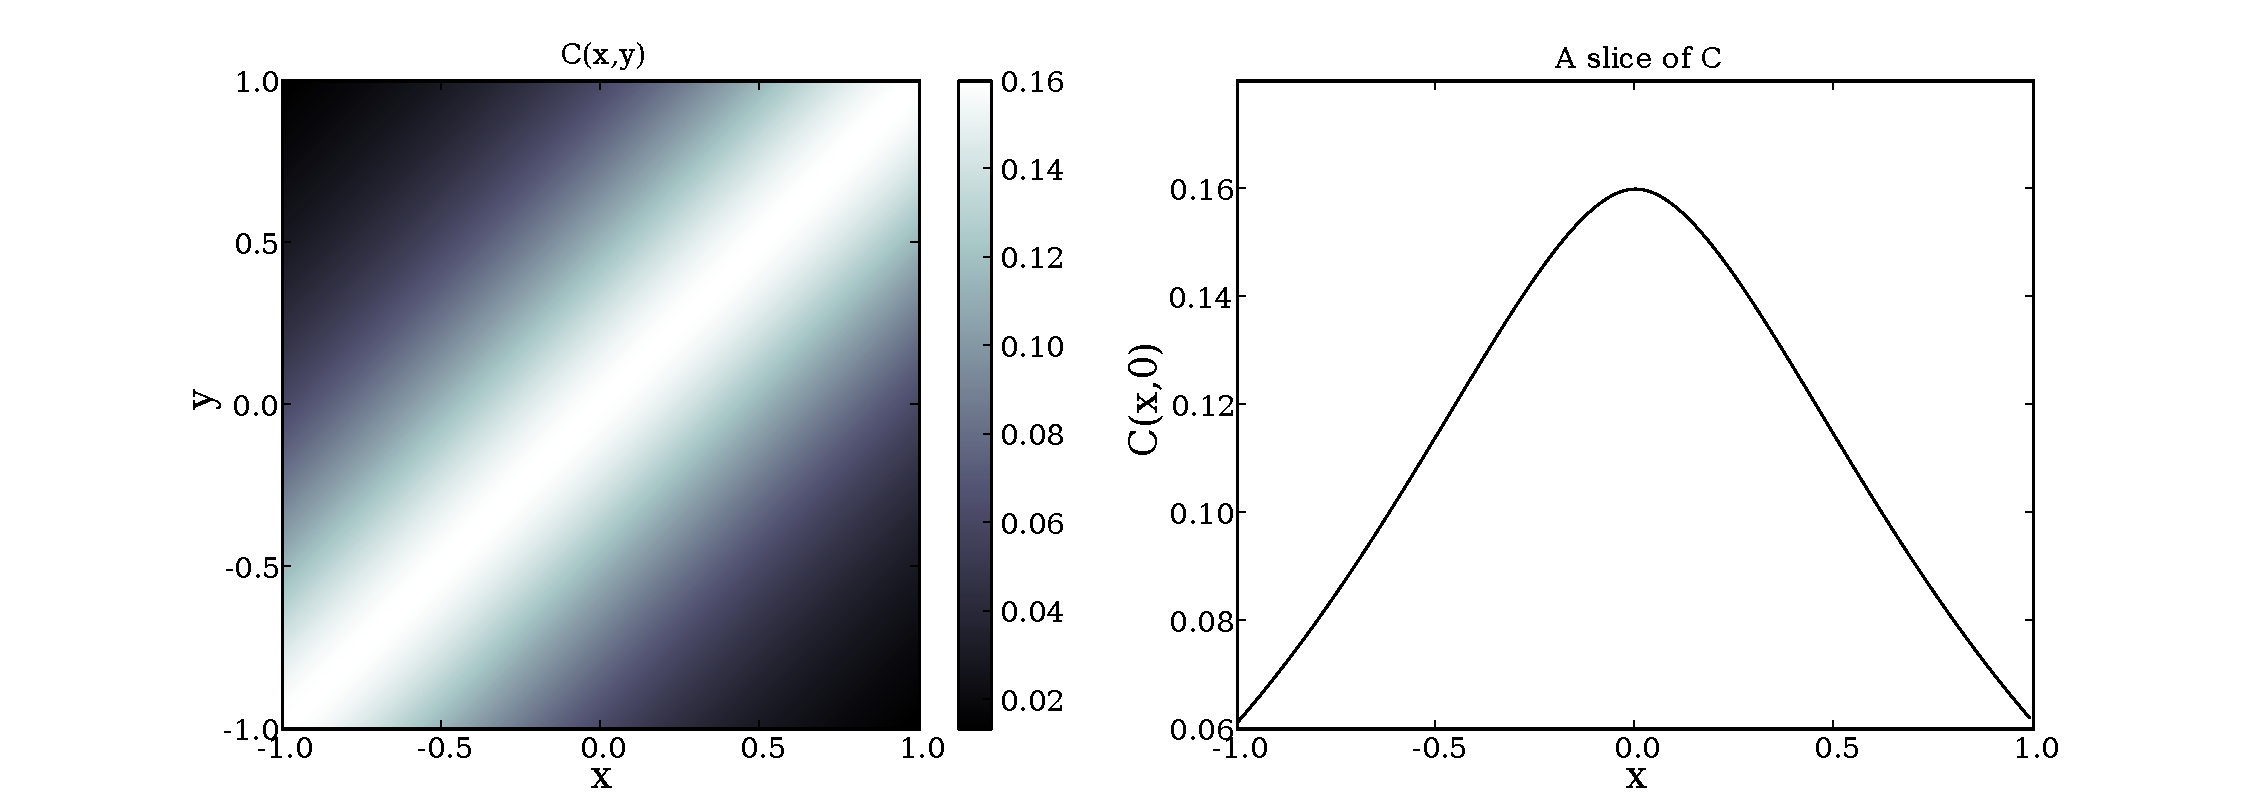
\epsfig{file=figs/cov.pdf,width=15cm}
	\caption{The covariance function generated by {\sffamily `examples/cov.py'}. On the left is the covariance function $C(x,y)$ evaluated over a square: $-1\le x\le 1,\ -1\le y\le 1$. On the right is a slice of the covariance: $C(x,0)$ for $0\le x \le 1$}
	\label{fig:cov}
\end{figure}

The first component of a GP that we will generate is a covariance function, which is represented by the class \class{Covariance}. The covariance function of a univariate GP is a function of two variables, and the \class{Covariance} class is a wrapper for an ordinary Python function of two variables. In this example we will use the popular Mat\'ern covariance function, which is provided in module \module{cov_funs}. In addition to the two variables, this function takes three tunable parameters: \code{amp} controls the amount by which $f$ may deviate from $M$, \code{diff_degree} controls the smoothness of $f$ (the degree of differentiability), and \code{scale} controls the wiggliness of $f$.

You're free to write your own covariance functions if you want, but not every function of two variables is acceptable as a covariance function. See section \ref{sec:usercov} for more information.

The code shown below will produce an instance of class \class{Covariance} called $C$. It will also display the covariance function $C(x,y)$ as a filled contour plot on the mesh ($-1<x<1$,$-1<y<1$).
\verbatiminput{../examples/cov.py}

The first argument, \function{eval_fun}, gives the Python function from which the covariance function will be made, in this case \function{Matern}. The \class{Covariance} class will raise an error if it is instantiated around an unacceptable function. The extra arguments \code{diff_degree, amp} and \code{scale} will be passed to \function{Matern}.

At this stage, the covariance function exposes a very simple user interface. In fact, it behaves a lot like its input function \function{Matern}. Try calling it. The only differences are: you only call it with $x$ and $y$ meshes, not with the extra arguments \code{diff_degree, amp} and \code{scale}; and you can just call it with one mesh, in which case it'll assume that the other mesh is the same and return a square matrix. Oh yeah- if you call it with array arguments, it'll return a matrix which gives it evaluated over all the values in the mesh. This behavior is handy. Input functions have to behave that way, too.

The last line plots the covariance as a filled contour plot evaluated on a mesh, which is shown in figure \ref{fig:cov}. You'll notice it looks like a band. The width of the covariance function band controls how tightly nearby evaluations of $f$ are coupled to each other. If there's a wide band, $f(x)$ and $f(y)$ will tend to have similar values when $x$ and $y$ are close to one another. If there's a narrower band, $f(x)$ and $f(y)$ won't be as tightly correlated. The height of the covariance function band controls the overall amplitude of $f$'s deviation from $M$. 

Try playing around with the parameters of \function{Matern} and see how $C$ changes.

\subsubsection{Instantiating a mean function}\label{subsub:mean}

\begin{figure}
	\centering
		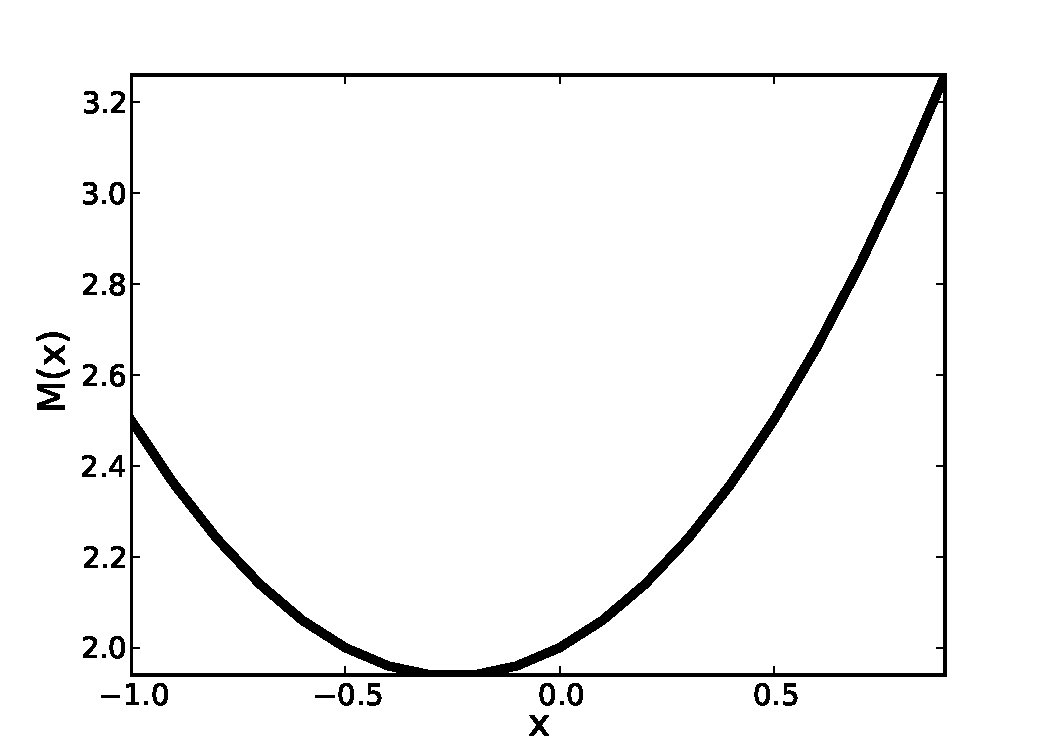
\epsfig{file=figs/mean.pdf,width=10cm}
	\caption{The mean function generated by {\sffamily `examples/meanAndCov.py'}.}
	\label{fig:mean}
\end{figure}

The second component we will generate is the mean function, represented by class \class{Mean}. The mean function of a univariate GP can be interpreted as a prior guess for the GP, so it's a univariate function also. Like \class{Covariance}, \class{Mean} is a wrapper for an ordinary Python function Unlike the covariance function however, there are no restrictions on the mean function; any function of one variable is fine. We will use the parabola
\begin{equation}
	M(x) = ax^2 + bx + c.
\end{equation}

The following code will produce an instance of class \class{Mean} called $M$, which will be associated with $C$. This association is unnecessary in this part of the tutorial, but it's essential for nonparametric regression and other conditioning operations, which we'll discuss later.
\verbatiminput{../examples/meanAndCov.py}

As with \class{Covariance}, the first argument to \class{Mean}'s init method is the underlying Python function, in this case \function{linfun}. The second argument, \code{C}, is the \class{Covariance} instance with which the mean function is associated. The extra arguments \code{a}, \code{b}  and \code{c} will be passed to \function{linfun}.

Like $C$, $M$ behaves a lot like its underlying, ordinary Python function. The last line plots $M(x)$ on $-1<x<1$, and its output is shown in figure \ref{fig:mean}. As expected, the plot is a parabola. 

Mean functions are much less magical than covariance functions, so it won't be as much fun to play with the parameters of \function{linfun}. As stated before, the mean function is just an initial guess for $f$.

\subsubsection{Drawing realizations}\label{subsub:realizations}
\begin{figure}
	\centering
		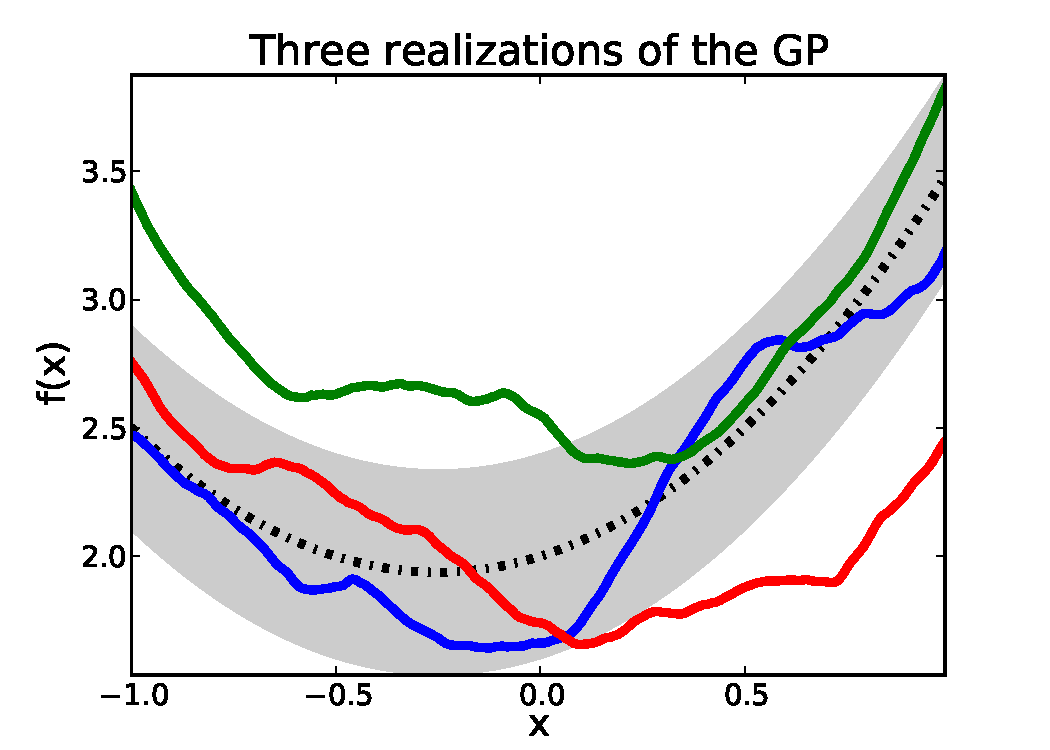
\epsfig{file=figs/realizations.pdf,width=10cm} 
	\caption{Three realizations from a Gaussian process displayed with mean $\pm$ 1 sd envelope. Generated by {\sffamily `examples/realizations.py'}.}
	\label{fig:realizations}
\end{figure}

Finally, let's generate some realizations (draws) from the Gaussian process defined by $M$ and $C$ and take a look at them. The following code will generate a list of instances of class \class{Realization} called \code{f_list}:
\verbatiminput{../examples/realizations.py}

The init method of \class{Realization} takes only two arguments, a mean function and a covariance function. Each element of \code{f_list} is a Gaussian process realization, which is a randomly-drawn function. Like ordinary numpy universal functions, GP realizations can be called with either values or ndarrays as arguments.

The third-to-last last line calls the function \function{plot_envelope}, which kind of summarizes the distribution. The dashdot black line in the middle is $M$, and the gray band is the $\pm 1$ standard deviation envelope generated by $C$. Each realization is a callable function, and their values over a mesh are plotted superimposed on the envelope. The plot output is shown in figure \ref{fig:realizations}. 

\subsubsection{Experiment!} 

As stated before, no matter how much math you know, the only way you'll be able to use GPs with confidence is by getting some experience with them. Now is a good time to have fun playing with the parameters of the mean and covariance functions. Change parameters of the covariance function, see how it looks using the code in section \ref{subsub:cov}, and try to guess how the realizations will look. See if you're right. Try generating $M$ around a different function. Try generating $C$ around one of the covariance functions from \module{cov_funs}, or if you're feeling adventurous try writing your own. 

% section firstlook (end)


\section{The role of the covariance function}\label{sec:cov} % (fold)

Various visualization methods of covariance, relationship between covariance's shape and differentiability of realizations.

% section cov_mean (end)


\section{Nonparametric regression: observing Gaussian processes}\label{sec:observing} % (fold)

\begin{figure}
	\centering
		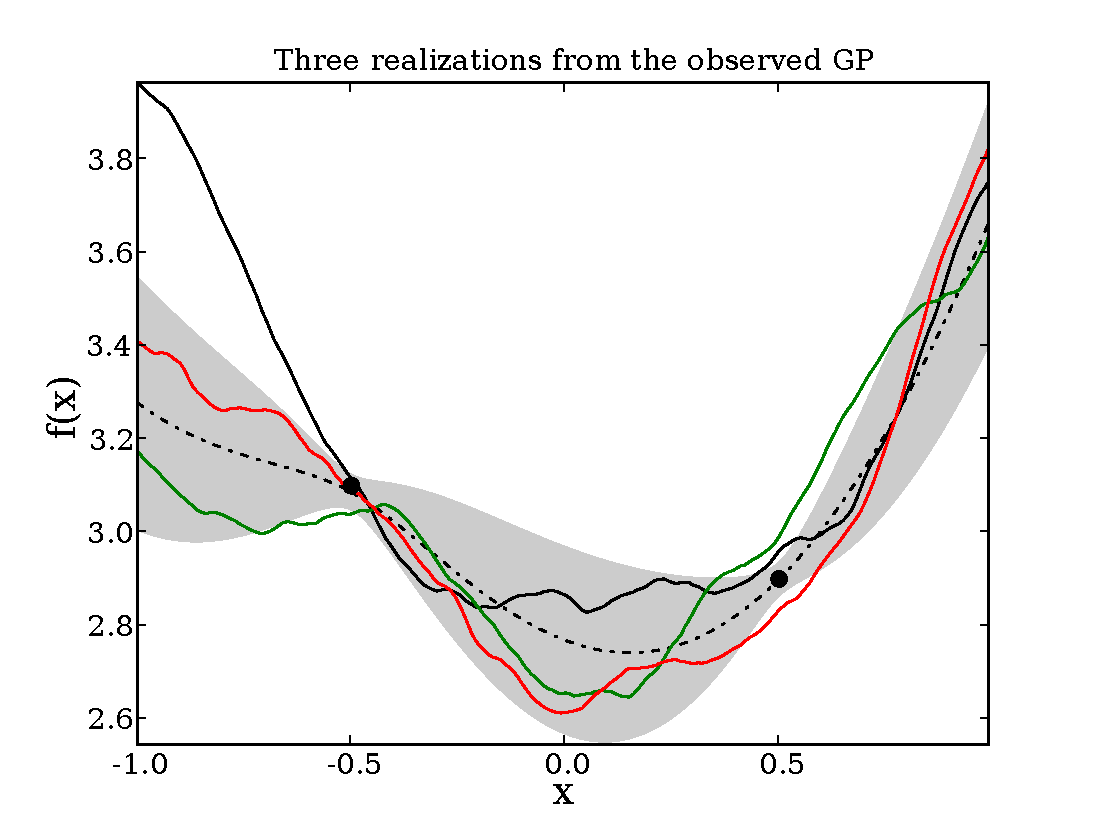
\epsfig{file=figs/obs.pdf,width=8cm}
		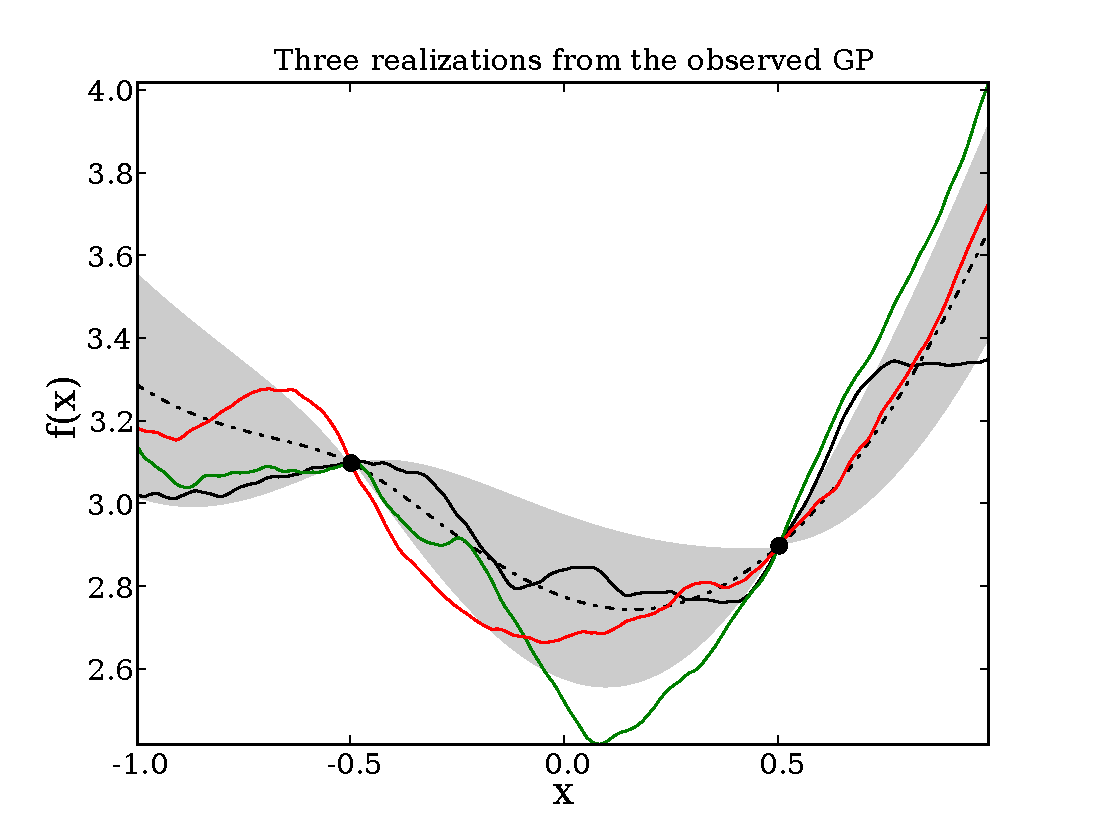
\epsfig{file=figs/cond.pdf,width=8cm}
	\caption{The output of {\sffamily `examples/observations.py'}: the observed (left) and conditioned (right) GP. Note that in the conditioned case, the $\pm$ 1 sd envelope shrinks to zero at the points where the observations were made, and all realizations pass through the observed values.}
	\label{fig:obs}
\end{figure}

Consider the following common statistical situation: You establish a prior for an unknown function $f$, then you observe the value of $f(x_i)$ at $N$ points, $\{x_i, i=0\ldots N-1\}$, possibly with uncertainty. If the observation error is normally distributed, it turns out that $f$'s posterior distribution given the new information is another Gaussian process. However, the new Gaussian process has different mean and covariance functions than $f$'s initial distribution.

This package provides a function called \function{observe} which allows you to impose normally-distributed observations on your Gaussian process. The following code imposes the observations
\begin{eqnarray}
	f(-.5) = 3.1, & \textup{observation precision}=500\\
	f(.5) = 3.1, & \textup{observation precision}=500
\end{eqnarray}
on the GP defined in \file{meanAndCov.py}:
\verbatiminput{../examples/observation.py} 

The function \function{observe} takes a covariance \code{C}  and (optionally) a mean \code{M} as arguments, and essentially tells them that their realizations' values on \code{obs_mesh} have been observed to be \code{obs_vals} with precision \code{obs_taus}. If \code{obs_taus} is \code{None}, \function{observe} assumes that the observation precision was infinite; that is, that the realizations' values on \code{obs_mesh} are known with no uncertainty. Making (or pretending to make) observations with infinite precision is sometimes called \emph{conditioning}, and can be a valuable tool for flexible GP construction; for example, if a rate function is known to be zero when a population's size is zero.

The output of the code is shown in figure \ref{fig:obs}, along with the output with \code{obs_taus=None}, so that the observation precision is infinite. Compare these to the analogous figure for the unobserved GP, figure \ref{fig:realizations}. The covariance after observation is visualized in figure \ref{fig:obscov}. The effect of observation was essentially to push the covariance down at the observation points. Very interesting.

Section \ref{sec:PyMC} will try to give you a deeper statistical understanding of observation and conditioning. 

\begin{figure}
	\centering
		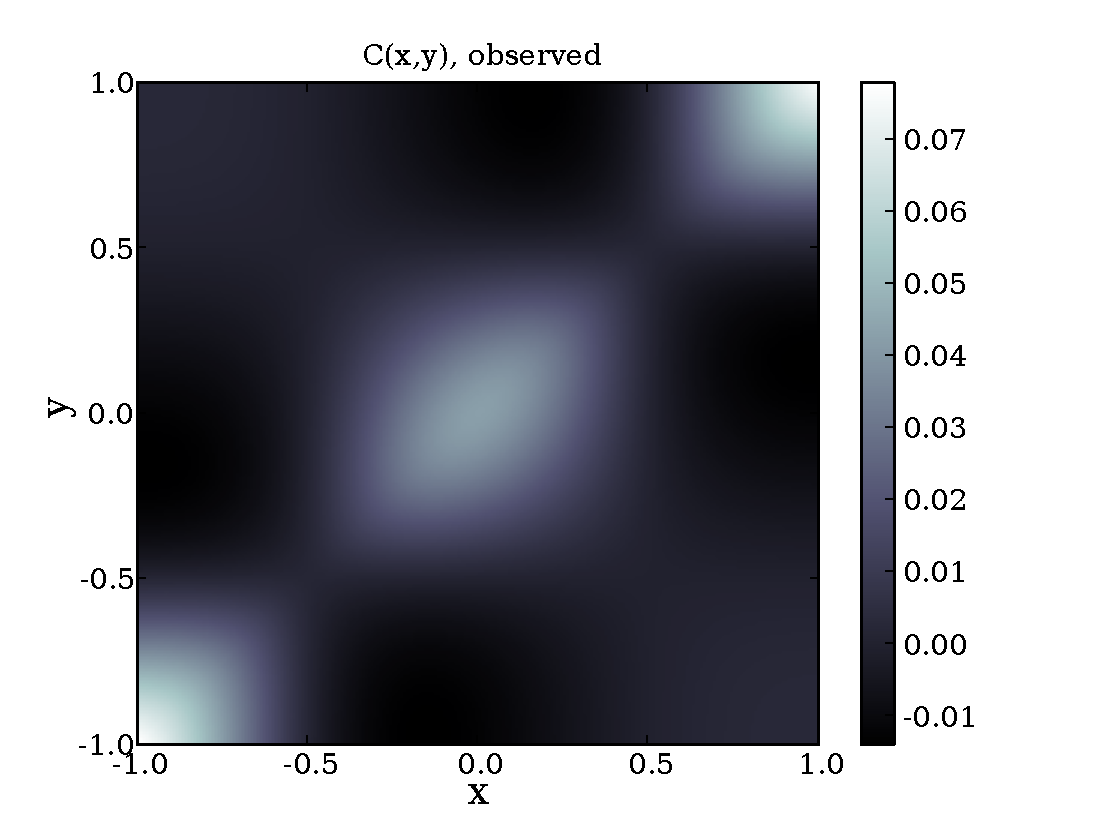
\epsfig{file=figs/obscov.pdf,width=10cm}
	\caption{The covariance function after observation. Compare this with the covariance function before observation, visualized in figure \ref{fig:cov} }
	\label{fig:obscov}
\end{figure}

We finally have the tools to partially reproduce Munch, Mangel and Kottas' results. \textbf{Nonparametric regression with fixed covariance parameters and mean parameters here. Show the stages of the covariance, with realizations: unconditioned, pegged at 0, observed at the datapoints. Note that this is better than MMK's results in some ways and worse in others: We've used Matern and pegged at 0, but have'nt allowed covariance parameters to vary. That'll have to wait for section \ref{sec:PyMC}.}
% section observing (end)


\section{The array aspect and performance}\label{sec:array} % (fold)
Conceptually, Gaussian process realizations are random functions, and the parameters of the Gaussian process are functions. To build intuition as quickly as possible, this tutorial has tried to stay faithful to the concepts by focussing on the functional aspect of \class{Covariance}, \class{Mean} and \class{Realization} as long as possible. 

From the package author's point of view, this was the hard part. Making \class{Realization} act like a function is particularly irritating; its return values have to be evaluated on-demand (lazily) using an algorithm whose expense increases with the number of calls made so far.

You may have noticed by now that \class{Covariance} is a subclass of \class{numpy.matrix}, and that \class{Mean} and \class{Realization} are subclasses of \class{numpy.ndarray}. That's because these objects are usually represented on a computer as arrays and matrices rather than functions. Certain properties of the Gaussian process distribution make this representation work well, though it requires a fair bit of linear algebra. 

Unfortunately, using the array representation of the Gaussian process is much faster than using the functional representation we have considered so far. If you need more performance from the Gaussian process than you've been getting, you may need to take a look at this section.

This section will try to introduce you to the array aspect of the GP, while insulating you from as much linear algebra as possible. The first subsection will tell you the bare minimum you need to know to use the array aspect, and subsequent sections will go into more depth.

\subsection{Utilitarian overview: the base mesh}

The init method of \class{Covariance} takes a parameter called \code{base_mesh}, which we haven't talked about yet. The base mesh is where you should put evaluations you know ahead of time you're going to want. The following code recreates the observed GP created in \file{examples/observation.py} and draws a single realization. However, this time a `base mesh' argument is provided.
\verbatiminput{../examples/basemesh.py}

The base mesh will be automatically inherited by $M$ and the realization $f$. We can do a few things now we couldn't do before.

\subsubsection{Indexing and slicing}\label{subsub:indexslice}
First, try typing the following command into the Python prompt, and you'll get the output below:
\begin{verbatim}
In [3]: print C
Gaussian process covariance
functional aspect: <function Matern at 0x496f4b0>
matrix aspect: ([[  7.78885868e-02,   6.60273508e-02,   4.99286671e-02,
                    3.22586177e-02,   1.53194936e-02,   1.48744121e-03,
                   -7.22296442e-03,  -1.18739011e-02,  -1.37398672e-02,
                   -1.36941495e-02,  -1.23668617e-02,  -1.02279152e-02,
                   ...
\end{verbatim}
$C$'s new `matrix aspect' is just $C$ evaluated on its base mesh. Try typing \code{print M} and \code{print f} into the prompt also. 

$C$ can still be called like a function, but now it can be treated like a matrix too:
\begin{verbatim}
In [11]: C(2.,3.)
Out[11]: matrix([[ 0.06014876]])

In [12]: C[3,:5]
Out[12]: matrix([[ 0.03225862,  0.03155917,  0.02869263,  0.02249194,  0.01228326]])

In [13]: isinstance(C,matrix)
Out[13]: True
\end{verbatim}
Similarly, $f$ and $M$ can still be called like functions, but now they can be treated like arrays:
\begin{verbatim}
In [14]: M(3)
Out[14]: array(12.506241348839085)

In [15]: f(3)
Out[15]: array(12.818659676751814)

In [16]: M[:5]
Out[16]: 
array([[ 3.27805131],
       [ 3.22089361],
       [ 3.18082649],
       [ 3.1518305 ],
       [ 3.12490149]])

In [17]: f[:5]
Out[17]: 
array([[ 3.22769661],
       [ 3.11578558],
       [ 3.07350289],
       [ 3.10476021],
       [ 3.09748845]])

In [18]: isinstance(M,ndarray)
Out[18]: True

In [19]: isinstance(f,ndarray)
Out[19]: True
\end{verbatim}


As you may have noticed, slicing (getting values from the array aspect) is much, much faster than calling (getting values from the functional aspect). If performance is a concern, you should make your base mesh include every value you're ever going to want, so that you don't have to make many calls at all. If that's not possible, you should keep the number of calls you make to a minimum. If you absolutely have to make a lot of calls but you still need high performance, consider a Fourier representation.
 
\subsubsection{Computing log-probabilities of realizations}\label{subsub:logp}
This module provides a function called \function{GP_logp} for computing the log-probability density of the evaluation of a realization $f$ on a base mesh, with respect to a mean function $M$ and a covariance function $C$. Try it out:
\begin{verbatim}
In [20]: GP_logp(f,M,C)
Out[20]: 39.2993852418

In [21]: GP_logp(2.*f,M,C)
Out[21]: -4667.56968213
\end{verbatim}
It looks plausible that $f$ is a realization from the GP defined by $M$ and $C$, but much less plausible that $2f$ is such a realization. This makes sense; $f$ really is a realization from that GP, but $2f$ would be way too far away from $M$ (see the $\pm$ 1 sd bands in figure \ref{fig:obs}, and imagine how ridiculous the realizations would look if they were doubled in amplitude).

If \function{GP_logp} is called with a realization $f$ that is way too ridiculous to ever have arisen from the GP, it raises a PyMC \exception{LikelihoodError} exception rather than returning \code{-Inf}. This is done for consistency with PyMC and for efficiency.

\subsubsection{Specifying realizations' values on the base mesh}\label{subsub:force}

The init method of \class{Realization} takes an argument we haven't used yet, called \code{init_base_array}. It allows us to force the realization to take particular values on the base mesh; that is, it allows us to force an array aspect on the realization. This is useful for proposing values in MCMC. We will defer further discussion of this feature until we need it in section \ref{sec:PyMC}. 

\subsection{The theory behind the array aspect} 
The Gaussian process generalizes the multivariate normal distribution from vectors to functions, just like the multivariate normal distribution generalizes the univariate normal distribution from scalars to vectors. The progression is as follows:
\begin{equation}
    \begin{array}{ll}
        y\sim\textup N(\mu,V): & \textup{$y$, $\mu$, $V$ are scalars}\\\\
        \vec y\sim\textup N(\vec \mu,C): & \textup{$\vec y$ and $\vec \mu$ are vectors, $C$ is a matrix}\\\\
        f\sim\textup{GP}(M, C): & \textup{$f$ and $M$ are functions of one variable, $C$ is a function of two variables}
    \end{array}
\end{equation}

One of the really nice things about this extended family of distributions is that it's easy to marginalize. For example, each element of a vector with a multivariate normal distribution has a univariate normal distribution:
\begin{eqnarray*}
    \vec y\sim\textup N(\vec \mu,C)\\
	\Rightarrow \vec y_i\sim\textup N(\vec \mu_i,C_{i,i}),
\end{eqnarray*}
and any subvector of a vector with a multivariate normal distribution has a multivariate normal distribution:
\begin{eqnarray*}
    \vec y\sim\textup N(\vec \mu,C)\\
	\Rightarrow \vec y_{i_1\ldots i_2}\sim\textup N(\vec \mu_{i_1\ldots i_2},C_{i_1\ldots i_2,i_1\ldots i_2}),
\end{eqnarray*}

This marginalizability applies to GP's as well. If $\vec x$ is a vector of values (a base mesh),
\begin{equation}
	\begin{array}{l}
		f\sim\textup{GP}(M, C)\\\\
		\Rightarrow f(\vec x) \sim\textup N(M(\vec x), C(\vec x,\vec x)).
	\end{array}
\end{equation}
In other words, the array aspect of a Gaussian process \class{Realization} has a multivariate normal distribution. Its mean is the array aspect of $f$'s associated \class{Mean} function, and its covariance is the matrix aspect of $f$'s associated \class{Covariance} function. 
% section array (end)

\section{Higher-dimensional GPs}\label{sec:highdim} % (fold)
Anytime you pass an array into an init method or evaluate a GP object on an array, the convention is that the array's last index iterates over spatial dimension. So if you wanted to evaluate a covariance function $C$ on the ordered pairs $(0,0)$, $(0,1)$, $(1,0)$ and $(1,1)$, you could pass in the following two-dimensional array:
\begin{verbatim}
[[0,0]
 [0,1]
 [1,0]
 [1,1]]
\end{verbatim}
or the following three-dimensional array:
\begin{verbatim}
[[[0,0]
  [0,1]],

  [1,0]
  [1,1]]]
\end{verbatim}
Either is fine, since in both the last index tells you which element of the ordered pair to use.

\textbf{A spatial example in 2d}
% section highdim (end)

\chapter{Tutorial II: More advanced topics}\label{cha:adv} % (fold)

\section{Incorporating Gaussian processes in probability models with PyMC}\label{sec:PyMC} % (fold)
\textbf{XXX Need to think about this a bit.}

You're NEVER allowed to change the base mesh. DON'T DO IT. I'll raise an error if you try.
% section PyMC (end)

\section{Integrals, derivatives and transforms: linear operations and constraints}\label{sec:linop} % (fold)

\textbf{XXX Not implemented yet. Maybe try to make a LinearOperator class. Define linear operations, talk about derivatives, integrals and Fourier transforms, how you can easily find their distribution. You can constrain the value of any linear operation, or softly constrain it. This is handy for building covariance functions. Introduce the \var{lintrans} argument. Maybe this shouldn't go in the tutorial.}

% section linop (end)

\section{Fourier representations, splines and convolutions}\label{sec:approx} % (fold)
Good if you need to make lots of calls, it's hard to establish a base mesh. Need to see how much can be implemented in time.

\subsection{Fourier representations}\label{sub:fourier}
\begin{itemize}
	\item Pros:
	\begin{itemize}
		\item Easy to go back and forth between Fourier and standard GP.
		\item Very solid and well-established theory.
		\item Straightforward to manipulate smoothness and wiggliness properties.
		\item Can often diagonalize covariance.
	\end{itemize}
	\item Cons:
	\begin{itemize}
		\item Harder for some people to visualize.
		\item Less standard in the field.
	\end{itemize}
\end{itemize}

\subsection{Splines}\label{sub:splines}
\begin{itemize}
	\item Pros \& cons: Need to ask Angela
\end{itemize}

\subsection{Convolutions}\label{sub:convolutions}
Need to look at Paciorek's thesis, see how much could be implemented in time.

% section fourier (end) 

\section{Writing your own covariance functions}\label{sec:usercov} % (fold)
If you want to write your own covariance function at some point, this module provides a function called \function{isPosDef} that can help you determine if your function is acceptable. It tests if a function is positive definite using Bochner's theorem. Also, \class{Covariance} will raise an error if it's able to determine that its underlying function is unacceptable, but it won't catch every unacceptable function. 

Three simple rules always apply to covariance functions, and keeping them in mind will reduce the amount of trial and error you have to go through:
\begin{itemize}
	\item $C(x,y)=C(y,x)$ for any $x$ and $y$.
	\item $C(x,x) \ge 0$ for any $x$.
	\item $C(x,x)\ge C(x,y)$ for any $x$ and $y$.
\end{itemize}

The theoretical condition is that the covariance has to be a symmetric nonnegative-definite function: its evaluation on any finite mesh has to be a symmetric nonnegative-definite matrix, which is a symmetric matrix whose eigenvalues are all nonnegative.

% section usercov (end)

% chapter adv (end)

\chapter{API reference}\label{cha:reference} 

Doxygen-style class reference here.


\end{document}
